\documentclass[
%aspectratio=169,
handout,
ignorenonframetext,hyperref={pdftex,unicode},xcolor=dvipsnames]{beamer}

\undef\C

\usepackage{amsmath,amssymb,amsthm,latexsym,color} %Basic packages
\usepackage{dsfont} % bb fonts for numbers
\usepackage{braket} % nice sets and more
\usepackage{accents}
\usepackage{musicography}
\usepackage{biblatex} % TODO: [citestyle=mla] causes compilation error
\usepackage{graphicx}
\usepackage[nice]{nicefrac}
\allowdisplaybreaks[2] %Allow page breaks in multi-line displays
\usepackage{xspace} % smart whitespacing after commands
\usepackage{mathtools}

%%%%%%%%%%%%%%%%%%%%%%%%%%%%%%%%%%%%%%%%%%%%%%%%%%%%%%%%%%%%%%%%%%%%%%
%Swaps the roles of phi and epsilon with the var versions
\let\temp\phi
\let\phi\varphi
\let\varphi\temp

\let\temp\epsilon
\let\epsilon\varepsilon
\let\varepsilon\temp
%%%%%%%%%%%%%%%%%%%%%%%%%%%%%%%%%%%%%%%%%%%%%%%%%%%%%%%%%%%%%%%%%%%%%%


%%%%%%%%%%%%%%%%%%%%%%%%%%%%%%%%%%%%%%%%%%%%%%%%%%%%%%%%%%%%%%%%%%%%%%
%Shorthand 
\newcommand{\seq}[1]{\{#1\}}
\newcommand{\linf}{\lim_{n \to \infty}}
\newcommand{\Alpha}{\mathcal{A}}
\newcommand{\ubar}[1]{\underaccent{\bar}{#1}}
\newcommand{\norm}[1]{\left\lVert#1\right\rVert}

\newcommand{\limnf}[1]{\liminf \limits_{#1}}
\newcommand{\limsp}[1]{\limsup \limits_{#1}}
\newcommand{\lone}{L^1}

\newcommand{\kph}{\ensuremath{\ket{\phi}}\xspace}
\newcommand{\kphind}{\ensuremath{\ket{\phi_i}}\xspace}
\newcommand{\kpho}{\ensuremath{\ket{\phi_0}}\xspace}
\newcommand{\kphi}{\ensuremath{\ket{\phi_1}}\xspace}
\newcommand{\kphii}{\ensuremath{\ket{\phi_2}}\xspace}
\newcommand{\ko}{\ensuremath{\ket{0}}\xspace}
\newcommand{\ki}{\ensuremath{\ket{1}}\xspace}
\newcommand{\koo}{\ensuremath{\ket{00}}\xspace}
\newcommand{\kio}{\ensuremath{\ket{10}}\xspace}
\newcommand{\koi}{\ensuremath{\ket{01}}\xspace}
\newcommand{\kii}{\ensuremath{\ket{11}}\xspace}

\newcommand{\Mod}[1]{\ (\mathrm{mod}\ #1)}

%%%%%%%%%%%%%%%%%%%%%%%%%%%%%%%%%%%%%%%%%%%%%%%%%%%%%%%%%%%%%%%%%%%%%%

%%%%%%%%%%%%%%%%%%%%%%%%%%%%%%%%%%%%%%%%%%%%%%%%%%%%%%%%%%%%%%%%%%%%%%
%Shorhands for commond blackboard bold symbols
\newcommand{\R}{\ensuremath{\mathbb R}}
\newcommand{\C}{\ensuremath{\mathbb C}}
\newcommand{\N}{\ensuremath{\mathbb N}}
\newcommand{\Q}{\ensuremath{\mathbb Q}}
\newcommand{\Z}{\ensuremath{\mathbb Z}}
%%%%%%%%%%%%%%%%%%%%%%%%%%%%%%%%%%%%%%%%%%%%%%%%%%%%%%%%%%%%%%%%%%%%%%

%%%%%%%%%%%%%%%%%%%%%%%%%%%%%%%%%%%%%%%%%%%%%%%%%%%%%%%%%%%%%%%%%%%%%%
%Used to alerting the reader
\newcommand{\nb}[1]{{\color{red}{$\clubsuit$#1$\clubsuit$}}}
%%%%%%%%%%%%%%%%%%%%%%%%%%%%%%%%%%%%%%%%%%%%%%%%%%%%%%%%%%%%%%%%%%%%%%

%%%%%%%%%%%%%%%%%%%%%%%%%%%%%%%%%%%%%%%%%%%%%%%%%%%%%%%%%%%%%%%%%%%%%%
%Theorem environments
\theoremstyle{definition}
\newtheorem{soln}{Solution}
\newtheorem{defn}{Definition}[soln]
\newtheorem{post}{Postulate}
\numberwithin{defn}{section}

\theoremstyle{plain}
\newtheorem{theo}{Theorem}[soln]
\newtheorem{prop}{Proposition}[soln]
\newtheorem{lem}{Lemma}[soln]
\newtheorem{claim}{Claim}[soln]
\newtheorem{cor}{Corollary}[soln]
\newtheorem*{exercise*}{Exercise}


\theoremstyle{remark}
\newtheorem{rem}{Remark}[soln]
\numberwithin{rem}{section}
%%%%%%%%%%%%%%%%%%%%%%%%%%%%%%%%%%%%%%%%%%%%%%%%%%%%%%%%%%%%%%%%%%%%%%



%%%%%%%%%%%%%%%%%%%%%%%%%%%%%%%%%%%%%%%%%%%%%%%%%%%%%%%%%%%%%%%%%%%%%%
\bibliography{citations}
%%%%%%%%%%%%%%%%%%%%%%%%%%%%%%%%%%%%%%%%%%%%%%%%%%%%%%%%%%%%%%%%%%%%%%

\usetheme{AnnArbor}
\usecolortheme{crane}
\useoutertheme{infolines}
\beamertemplatenavigationsymbolsempty
\usealerttemplate{\color{red}}{}

\AtBeginSection[]
{
\begin{frame}<beamer>
\frametitle{Outline}
\tableofcontents[currentsection,hideothersubsections]
\end{frame}
}

\AtBeginSubsection[]
{
\begin{frame}<beamer>
\frametitle{Outline} 
\tableofcontents[currentsection,subsectionstyle=show/shaded/hide,subsubsectionstyle=show/shaded/hide]
\end{frame}
}

\newcommand{\screenshot}[1]{
\begin{center} 
\includegraphics[width=12cm,keepaspectratio]{./pics/#1}
\end{center}
}

\newcommand{\screenshotw}[2]{
\begin{center} 
\includegraphics[width=#1,keepaspectratio]{./pics/#2}
\end{center}
}

\BeforeBeginEnvironment{frame}{%
  \setlength{\abovedisplayshortskip}{2mm}
  \setlength{\belowdisplayshortskip}{1mm} 
  \setlength{\abovedisplayskip}{2mm}
  \setlength{\belowdisplayskip}{1mm} 
}

\begin{document}

\begin{frame}{Outline}
\tableofcontents
\end{frame}


\section{Section: Introduction}

\subsection{History}

\begin{frame}{Founding Fathers}

  Time: early 1980-s

  People: Paul Benioff, Richard Feynman, and Yuri Manin

  \vspace{.3cm}

  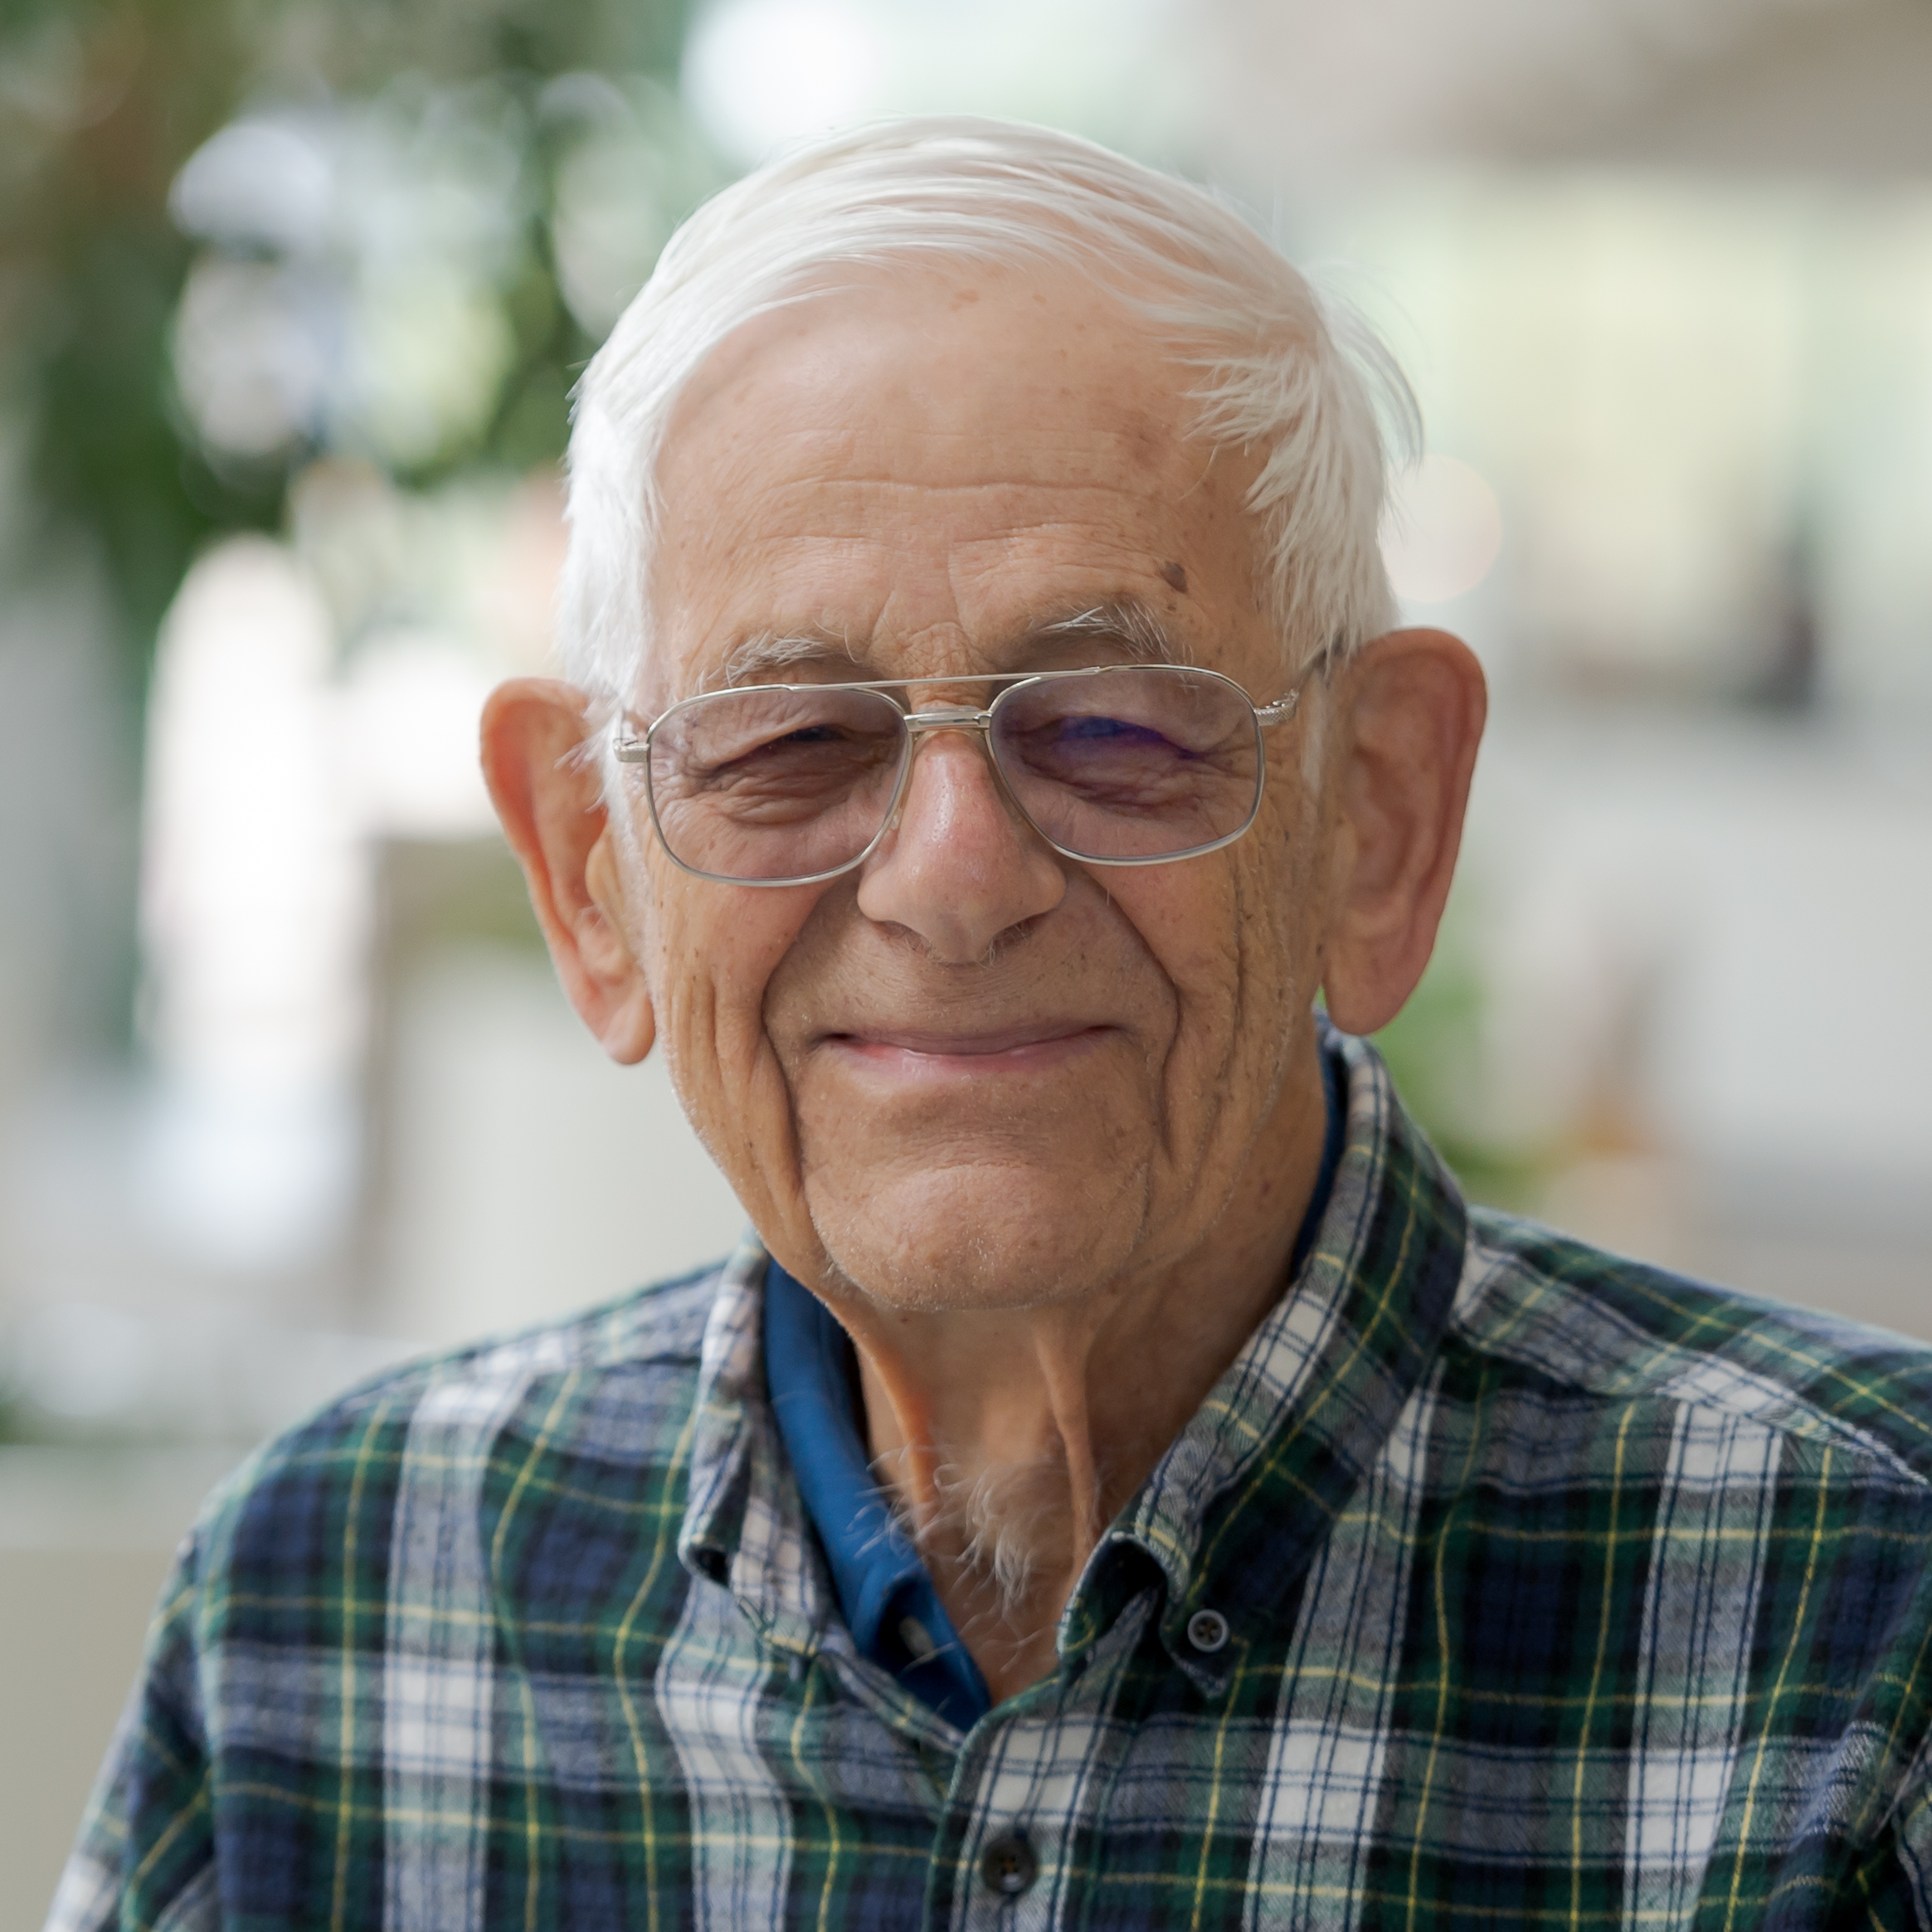
\includegraphics[width=3.6cm]{./pics/benioff.jpg}
  \hfill
  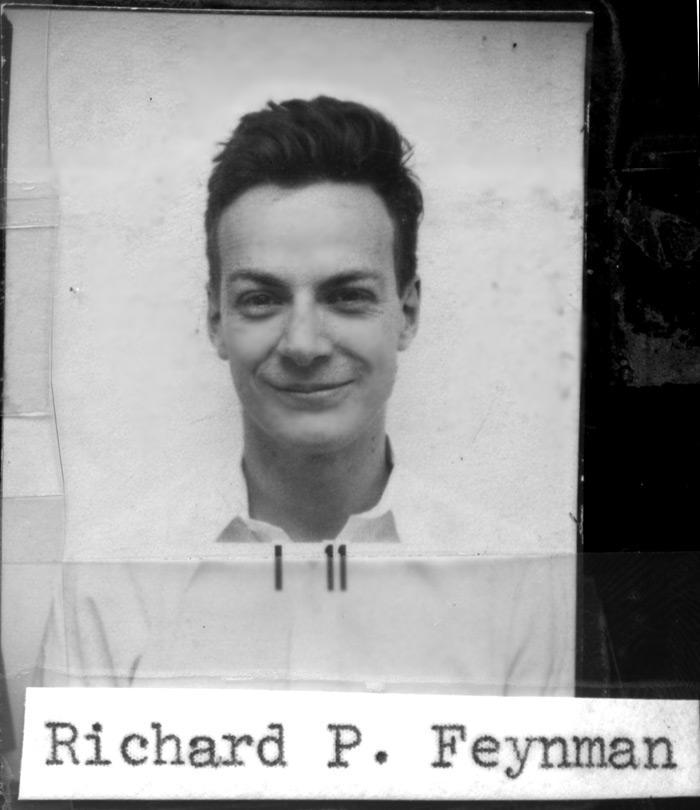
\includegraphics[width=3.6cm]{./pics/feynman.jpg}
  \hfill
  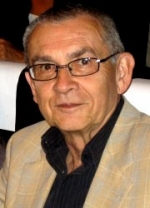
\includegraphics[width=2.9cm]{./pics/manin.jpg}

  \pause
  \vspace{3mm}
  Key Tool: \alert{Quantum Parallelism} \pause (tricky to employ)

\end{frame}

\subsection{Significance}

\begin{frame}{The Pearl: Shor's Algorithm (1994)}

  \vspace{5mm}
  Problem: Integer Factorization

  \vspace{5mm}
  Best ``Classical'' Solution:
    $ O \! \left( e^{1.9 (\log N)^{1/3} (\log \log N)^{2/3}} \right)$
    
  \vspace{5mm}
  Shor's Algorithm:
    $O \! \left( (\log N)^{2} (\log \log N) (\log \log \log N) \right)$

\end{frame}


\section{Section: Computational Model}

\subsection{Quantum Information}

\begin{frame}{State Space Postulate}
\pause
  \begin{block}{Postulate 1 (State Space Postulate)}
  The state of a system is described by a unit vector in a Hilbert space $\mathcal H$.
  \end{block}

  \pause

  \begin{columns}
  \column{5.4cm}

    \begin{block}{``Systems''}
      A piece of physical reality used to encode information akin to trnsistors, e.g.
      \begin{itemize}
      \item electron and its spin,
      \item photon and its polarization,
      \item spins of other particles
      \end{itemize}

    \end{block}

  \column{5.4cm} \pause  
  
    \begin{block}{Hilbert space}
      Complex \textbf{vector space} with a\\\textbf{scalar product}
      \\
      (to measure angles and lengths).
      
      \pause
      \vspace{7mm}
      Once you pick a basis, its basically $\C^n$.
    \end{block}
  
  \end{columns}


  \pause
  \begin{block}{Example: 2 dimensions, fixed basis: \ko, \ki $\Rightarrow$ \alert{qubit}}
  \[
    \alpha_0 \ket 0 + \alpha_1 \ket 1, \qquad 
    \alpha_i \in \C: |\alpha_0|^2 + |\alpha_1|^2 = 1.
  \]
  \end{block}

\end{frame}

%\subsubsection{Composite Systems}

\begin{frame}{Composite Systems}

  \begin{block}{Composition of Systems Postulate}
  If one system is in the state \kphi and the second system in the state 
  \kphii, then the state of the combined system is described by the 
  \emph{tensor product}:
  \[
      \kphi \otimes \kphii \in \mathcal H_1 \otimes \mathcal H_2,\qquad \text{if }
      \ket{\phi_i}\in\mathcal H_i.
  \]
  \end{block}

  \pause
  \textbf{Notation} Instead of $\kphi \otimes \kphii$ we write \kphi\kphii or even $\ket{\phi_1\phi_2}$.

  \pause
  \vspace{3mm}
  Tensor Product in a Nutshell: bilinear pairing operation.

  \pause
  \begin{block}{Example: two qubits}
  Given
  \[
    \kphi = \nicefrac 1 {\sqrt 2} (\ko + \ki), \qquad 
    \kphii = \nicefrac 1 {\sqrt 2} (\ko - \ki).
  \]
  their composite is described with:\pause \hfill \onslide<6>{\alert{What about dimension?}}
  \[
    \kphi \kphii = \nicefrac 1 2 (\ko + \ki) (\ko - \ki) 
      = \nicefrac 1 2 (\ket{00} - \ket{01} +\ket{10} +\ket{11}).
  \]
  \end{block}

\end{frame}


\begin{frame}{Entangled States}
  Can we always un-tensor states of two qubits?

  \pause
  \vspace{5mm}
  No (...t at all):
  \[
    \kph = \nicefrac 1 {\sqrt 2} ( \koo + \kii )
  \]

  \pause
  Fancy name: \alert{EPR pair} (for Einstein, Podolsky, and Rosen)

\end{frame}



\subsection{Quantum Transformations}

\begin{frame}{The Way To Compute}

  What to require from a computational tool when work with \emph{unit vectors}?

  \pause

  \begin{block}{Evolution Postulate}
    The time-evolution of the state of a closed quantum system is described
    by a \alert{unitary operator}: 
    $\exists U\colon  \ket{\phi_{t0+x}} = U \ket{\phi_{t0}}$.
  \end{block}
  
  \pause
  
  \begin{columns}
  \column{5.4cm}

    \begin{block}{Unitary Operators}
      \vspace{-4mm}
      \[
        U \text{— unitary} \Leftrightarrow (Ux,Uy) = (x,y).
      \]
      %
      \pause
      Using adjoint opertor:
      \[
        (Ux,Uy) = (x,U^*Uy),
      \]
      an equivalent formulation:
      \[
        U \text{— unitary} \Leftrightarrow U^*=U^{-1}.
      \]

    \end{block}


  \column{5.4cm} \pause  
  
    \begin{block}{Case of Real-Valued Matrices}
    First, $U^*$ is simply $U^T$. 
      \[
        U \text{— unitary} \Leftrightarrow U^{-1}=U^T.
      \]
    %So $U$ is unitary if its inverse is given by its transposition.
    
    Second, if an operator is self-inverse ($U^{-1}=U$), then 
      \[
        U \text{— unitary} \Leftrightarrow U=U^T.
      \]
    \end{block}
  
  \end{columns}
  
\end{frame}

\subsection{Measurement}

\begin{frame}{The Cats Of It}
  \begin{block}{Problem: Can't Access The Amplitudes}
    A ``classical'' observer can only get to basis states, e.g. \ko, \ki.

    So what do superposition states mean?
    \[
      \text{cat: } \nicefrac 1 {\sqrt 2} \text{ dead} + \nicefrac 1 
    {\sqrt 2} \text{ alive}...
    \]
  \end{block}
  
  \pause
  \begin{block}{Measurement Postulate}
    Consider a system $A$ and its state space $\mathcal H_A$.
    
    For an orthonormal basis $B = \seq{\kphind}$ in $\mathcal H_A$, there exists
    a description of $A$:
    \[
        \kph = \sum_i \alpha_i\kphind, \qquad \sum_i |\alpha_i|^2 = 1.
    \]
    \pause
    It is possible to perform a \emph{(Von Neumann) measurement} on 
    system $A$ with respect to the basis $B$. With probability $|\alpha_i|^2$, 
    this act outputs a label $i$ and leaves the system in state \kphind.
  \end{block}
  
\end{frame}

\begin{frame}{Measurement Examples}

  \vspace{-6mm}
  \[
    \kph 
    = \sqrt{\nicefrac 1 {11}} \koo 
    + \sqrt{\nicefrac 5 {11}} \koi
    + \sqrt{\nicefrac 2 {11}} \kio
    + \sqrt{\nicefrac 3 {11}} \kii
  \]

  \pause
  \begin{block}{Measure both qubits}
    What are the possible outcomes of measuring the pair of qubits?

    \pause
    Here they are:
    \begin{itemize}
      \item 00 --- with probability $\nicefrac 1 {11}$; the system turns into \koo
      \item 01 --- with probability $\nicefrac 5 {11}$; the system turns into \koi \hspace{1cm} ...
    \end{itemize}
  \end{block}

  \pause
  \begin{block}{Measure the first qubit}
    \setlength{\abovedisplayskip}{1mm}
    \setlength{\belowdisplayskip}{-3mm} 
    \setlength{\abovedisplayshortskip}{1mm}
    \setlength{\belowdisplayshortskip}{-1mm} 

    \textit{Note from above}:\\
    the probability of getting $0$ for the first qubit is $\nicefrac 1 {11} + \nicefrac 5 {11} = \nicefrac 6 {11}$.

    \pause
    So, we factor out $\sqrt{\nicefrac 6 {11}}$ first to get:
    \[
      \kph 
      = \sqrt{\nicefrac 6 {11}} \ko \left ( 
        \sqrt{\nicefrac 1 6} \ko + \sqrt{\nicefrac 5 6} \ki
      \right ) +
      \sqrt{\nicefrac 5 {11}} \ki \left ( 
        \sqrt{\nicefrac 2 5} \ko + \sqrt{\nicefrac 3 5} \ki
      \right ).
    \]
    \pause
    \[
      \text{When output=0 the system becomes: }
      \onslide<7>{
      \ko ( 
        \sqrt{\nicefrac 1 6} \ko + \sqrt{\nicefrac 5 6} \ki
       ).}
    \]
  \end{block}

\end{frame}


\section{Section: Quantum Algorithms}

\begin{frame}{The Road to Shor}

  \pause
  \begin{block}{Idea 1 (a simple one)}
    We only need to be able to find one factor of the input $N$.
  \end{block}

  \pause
  \begin{block}{Idea 2 (a technical one)}
    Take random $A < N$ coprime to $N$. An integer $r$ is called the 
    \alert{order} of $A$ modulo $N$ if
    $A^r \equiv 1 \Mod N$.
    
    \pause
    Finding a factor of $N$ can be efficiently reduced to the 
    order-finding problem.
  \end{block}

  \pause
  \begin{block}{The Insight About Periodicity}
    The order-finding problem can be seen as the problem of finding the
    period of the following mapping:
    \[
      \exp_{A,N}\colon \quad b \mapsto A^b \Mod N, \qquad \text{where } b\in\Z.
    \]
  \end{block}

\end{frame}

\begin{frame}{Periodic Functions: What and Why}

  \begin{block}{Definition}
    $f\colon G \to X$ defined on a group $G$ 
    is \emph{periodic with period} $r\in G$ ($r\neq e$) if:
    \[
       \forall n\in\Z\: \forall g\in G\colon f(g+rn) = f(g).
    \]
  \end{block}

  \pause
  \begin{block}{Shor's Problem}
    Find the period of a particular function ($\exp_{A,N}$) defined on the group \Z.
    
    {\small\emph{Note}: In fact, on a smaller group, $\Z_{\phi(N)}$, but we don't 
    know it in advance, hence the other name: the \emph{hidden subgroup problem}.}
  \end{block}

  \pause
  We are in rush, so we tackle an easier instance of the same problem.
  \begin{block}{Simon's Problem}
    Find the period of a function defined on the group $\Z^n_2$.    
  \end{block}

\end{frame}

\begin{frame}{Simon's Problem}

  \begin{block}{Formulation}
  \textbf{Input:} A black-box for computing an unknown function $f\colon \Z^n_2 \to X$.\\
  \textbf{Promise:} There exists $\bar s$, s.t.: $f(\bar x) = f(\bar y)$ iff $\bar x = \bar y$
  or $\bar x = \bar y \oplus \bar s$.
  \textbf{Problem:} Determine $\bar s$ by making queries to $f$.
  \end{block}

  \pause
  \begin{block}{The Circuit}
  \screenshotw{9cm}{simon.pdf}
  
  \pause
  \vspace{-1cm}
  \[
      \ket {0^{2n}} 
        \xmapsto{(1)} \pause
          \sum_{\bar x \in \Z^n_2} \ket {\bar x \,0^n}
        \xmapsto{(2)} \pause
          \sum_{\bar x \in \Z^n_2} 
            \ket {\bar x} \ket{f(\bar x)}
        \xmapsto{(3)} \pause %\sum_{\bar x \in I} 
          (\ket {\bar x} + \ket {\bar x \oplus \bar s}) \ket{f(\bar x)}
        \xmapsto{(4)} \ldots
  \]
  \end{block}

\end{frame}


\begin{frame}{Why The Circuit Works (And What it Outputs)}

  \begin{block}{Hadamard on a coset}
  \[
    H^{\oplus n}(\ket{\bar x} + \ket{\bar x \oplus \bar s}  ) =
      \sum_{\bar z \in {\bar s}^\perp} (-1)^{\bar x \cdot \bar z} \ket{\bar z}.
  \]
  \end{block}

  \pause
  \begin{block}{Output of The Circuit}
  Claim: the output on the first $n$ wires of the circuit is a vector $\bar z \in {\bar s}^\perp$.
  \end{block}
  
\end{frame}

\section{Conclusions}

\begin{frame}{Quantum Computing}

\begin{itemize}[<+->]
\item Massively data-parallel model with probablistic outcomes;
\item good only for certain classes of tasks,\\
      esp. when searching for global properties of functions;
\item some of the applications are very important (e.g. in cryptography);
\item practise lags behind theory.
\end{itemize}

\end{frame}


\end{document}

\begin{frame}{Slide 1}
  \begin{block}
  \end{block}

\end{frame}

  \begin{block}{}
  \end{block}

%~ \begin{itemize}
%~ \item 
%~ \end{itemize}
